\chapter{Research methodology}
\label{ch:res_metho}
\rrod{Define research questions}
\rrod{Discuss main research question}
\rrod{Define research boundaries}
\rrod{Define project goals}
\rrod{Implement scanner descision, became research question, will be answered in SR.}
\rrod{Use limitations of phantoms to lead to research question}

Different perfusion phantoms have been developed. Some are specifically designed to simulate the myocardial perfusion \footnote{\citep{chiribiri2013perfusion, otton2013direct, o2017effect, o2017feasibility, teslow1991x}}, others for brain perfusion \footnote{\citep{hashimoto2018effect, suzuki2017quantitative, boese2013performance, mathys2012phantom, ebrahimi2010microfabricated, wang2010flow, noguchi2007quantitative, ganguly2012vitro, klotz1999perfusion}}, or capillaries in general \footnote{\citep{kim2016efficiency, anderson2011semipermeable, driscoll2011development, gauthier2011perfusion, veltmann2002design, lohmaier2004vitro}}, and even phantoms to simulate perfusion in rheumatoid finger joints \citep{sakano2015power} and skin \citep{kim2018multidimensional}. Most software packages are designed for human organs and look for landmarks such that it can perform the most optimal calculation. Many of these phantoms do not resemble human anatomy. The phantom proposed by \cite{chiribiri2013perfusion}, the four-chambered heart, comes close to mimicking a human heart. However, the myocardium chamber is simplified and not covering the chambers. Furthermore, the phantoms are unable to mimic cardiac defects. These anatomical anomalies, and the inability to mimic cardiac defects,  results in the need for a new phantom.

\section{Research questions}
\begin{figure}[b!]
	\begin{center}
		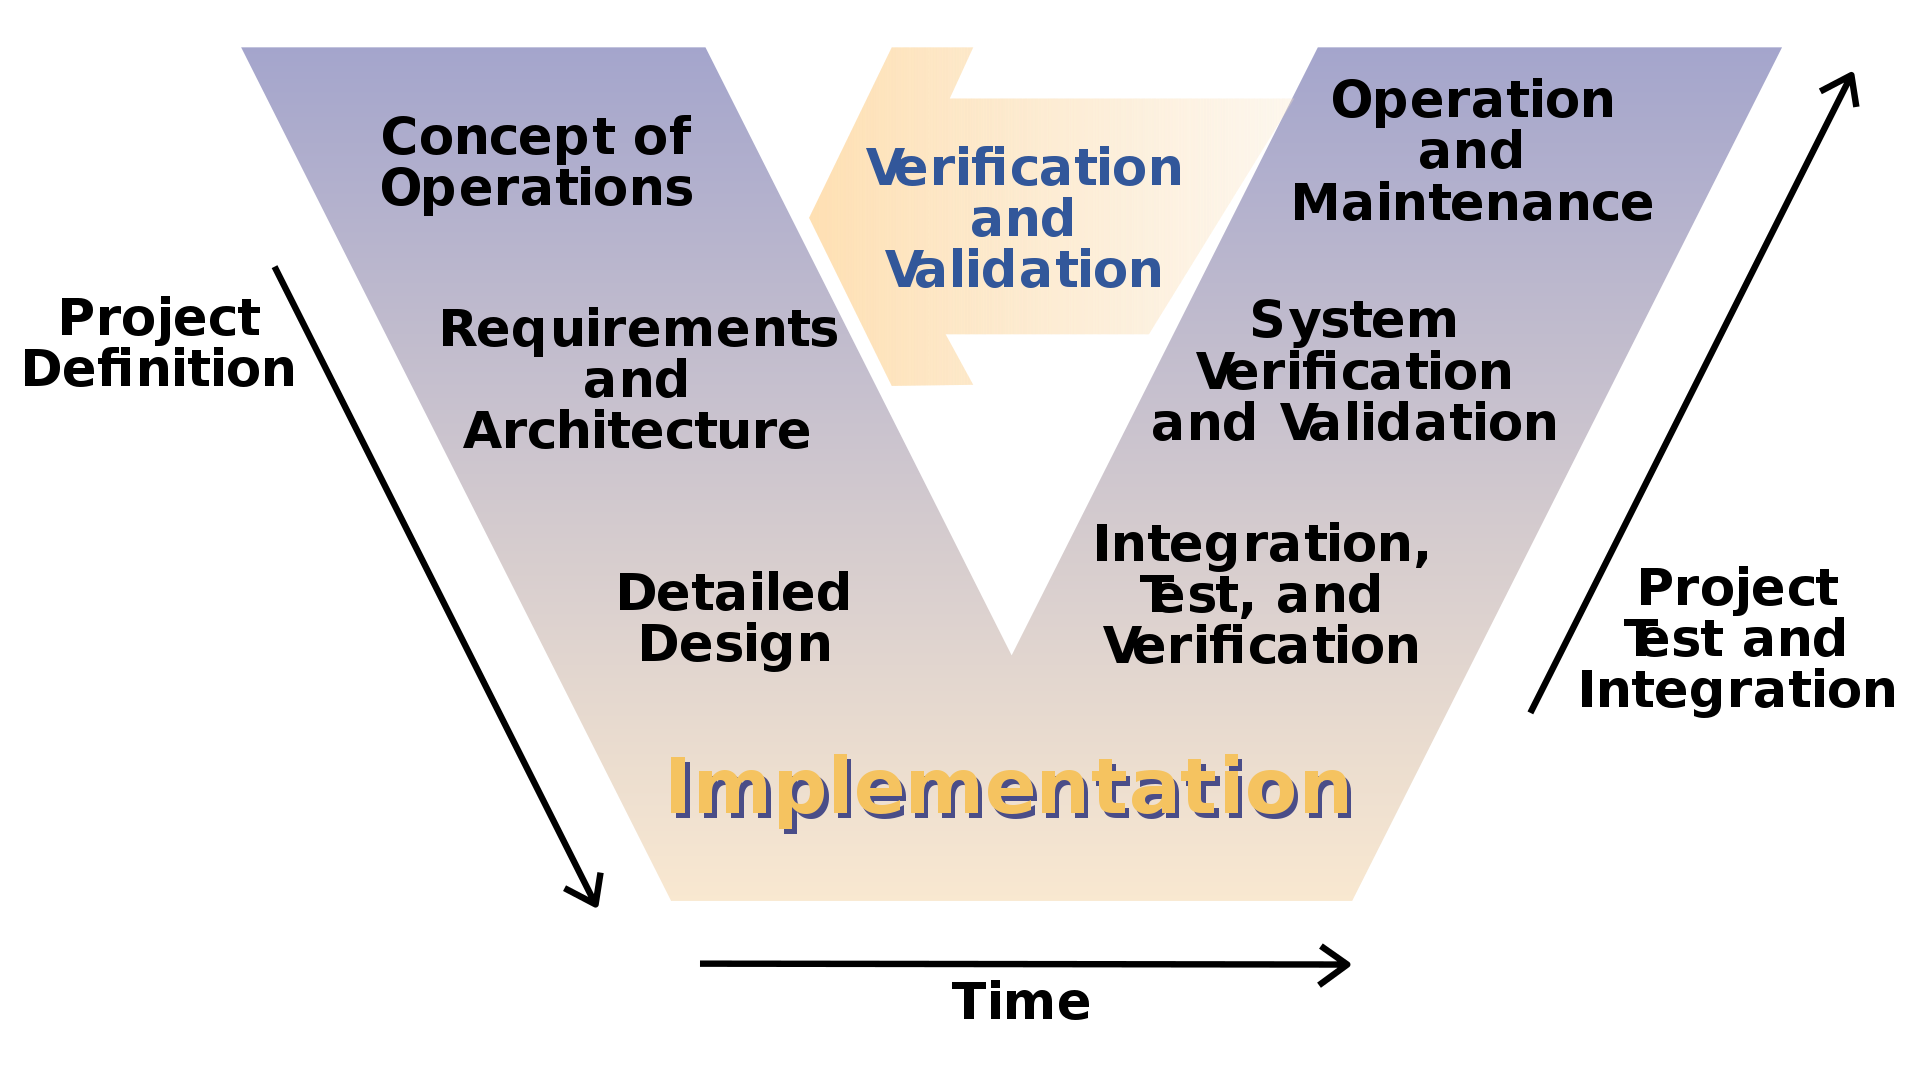
\includegraphics[width=0.5\linewidth]{images/vmodel.png}
	\end{center}
	\caption{V-Model\citep{rook1986controlling} as proposed by \cite{osborne2005clarus}}
	\label{fig:vmodel}
\end{figure}
Can patient treatment reliably depend on the D-SPECT, using dynamic scanning, in myocardial perfusion imaging?

\subsection{Primary goal}
The goal of the project is to develop a prototype myocardial perfusion phantom capable of reproducible simulations of typical and cardiac defect situations using clinical software commonly used in myocardial perfusion scans. Most software packages require anatomical landmarks which imposes requirements on the phantom. In addition, the phantom can be used for educational and training purposes to demonstrate the impact of (poorly) chosen variables, e.g. pressure or flow, scanning parameters, cardiac defects, and so forth.

The primary goal is not to validate the D-SPECT, but to design and build a tool for that validation purpose. The project itself is carried out using the V-Model \citep{rook1986controlling,osborne2005clarus} approach, see figure \ref{fig:vmodel}. Sub-research questions are based on this V-Model approach such that each phase has its own goal.

\subsection{Concept of operations}
Is the D-SPECT's dynamic scanning, in comparison with other modalities (CT, MRI, PET, or SPECT), suitable for quantitative myocardial perfusion imaging?

What must the myocardial perfusion phantom be able to simulate?

\subsection{Requirements and Architecture}
What are the requirements for a myocardial perfusion phantom that can be used in combination with commonly used clinical software?

\subsection{Detailed Design}
How can the myocardial perfusion phantom meet the clinical requirements and mimic the perfusion of a human heart?

\subsection{Implementation and verification}
Does the prototype myocardial perfusion phantom meet the specified requirements? 

\subsection{Secondary goal}
During the individual project, a calibration set-up for flow and pressure sensors has been developed. The prototype version showed that flow sensors can be calibrated using the "emptying tank" principle. Pressure sensors have not been implemented in the prototype. Furthermore, the calibration set-up relies too much on human interaction. A sub-goal of the project will be to improve the existing calibration set-up such that flow and pressure sensors can be calibrated which in turn will increase the reliability of the flow set-up.

\section{Stakeholders}
\label{sec:stakeholders}
A distinction is made between direct stakeholders, actively involved in the development, indirect stakeholders, can provide knowledge or resources, and beneficial stakeholders, (potentially) benefit from the development.

\begin{tabular}{lll}
 	\multicolumn{1}{c}{\textbf{Direct}} & \multicolumn{1}{c}{\textbf{Indirect}} & \multicolumn{1}{c}{\textbf{Beneficial}} \\
	 - C.H. (Kees) Slump, &  - M.J.W. (Marcel) Greuter, & - Patients with suspected \ac{CAD}, \\
	 - M.E. (Marije) Kamphuis, & - R.H.J.A. (Riemer) Slart, & - Scanner manufacturers,\\
	 - Clinical Physicists, & - W.L. (Willem) van Meurs. & - Scanner software developers, \\
	 - Lab technicians, & & - Hospitals, \\
	 - Nuclear Medicine Physicians, & & - Physicians.\\
	 - Cardiologists. & & \\
\end{tabular}

\section{Approach}
The research questions will primarily be answered by means of literature and by interviews with the stakeholders, see section \ref{sec:stakeholders}. They are regularly involved with myocardial perfusion imaging and are thus familiar with the clinical software, hardware, work flow, and requirements. These interviews will provide additional (practical) insight.

Part of the V-Model approach is the continuous feedback. Requirements and designs are constantly updated according to new insights acquired during the development process. 

\subsection{General concept}
\begin{figure}[b!]
	\begin{center}
		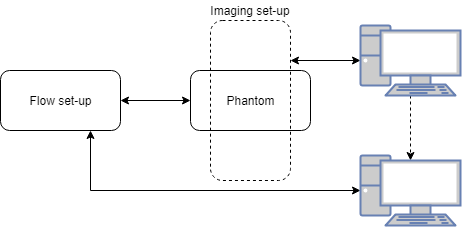
\includegraphics[width=0.75\linewidth]{images/global_setup.png}
	\end{center}
	\caption{General concept, schematic}
	\label{fig:general_concept}
\end{figure}
A general concept is shown in figure \ref{fig:general_concept}. Three main parts can be identified: flow set-up, phantom, and imaging device. The flow set-up consists of everything to produce and maintain pressures and/or flows and measure these variables. The user-interface is a computer or laptop. The phantom consist of everything needed to mimic cardiac defects and to provide a representative image for myocardial perfusion image processing software. The imaging set-up consists of the imaging device itself along with any contrast agents needed to properly image the phantom. Many imaging devices communicate with a dedicated workstation on which the image processing software runs.

\section{Boundaries}
The project is carried out as an Electrical Engineering's final thesis project of 40 \ac{ECTS}. The boundaries for the project is to design and build a flow phantom capable of simulating myocardial blood flow according to specified, and agreed upon, system requirements. These system requirements require research, interviews and knowledge on physiology and are thus part of the project. The phantom and its set-up are part of research performed by M.E. (Marije) Kamphuis and imposes additional requirements on the project. The project is a tool for Marije to answer her research questions, but answering these research questions is not part of the final thesis. 

\section{Additional resources}
During the individual project of G.J. (Gijs) de Vries, a prototype flow set-up, control module, and calibration set-up has been realised and can be used / re-cycled.
\subsection{Flow set-up}
The flow set-up uses simple, low costs pumps and available flow sensors. These might not be suitable for high precision flow systems. It is encouraged to look into alternatives.
\subsection{Control module}
The control module requires improvement when it is to be re-used. Two of the main improvements consist of improving the electro(magnetic) shielding to decrease the susceptibility to noise and to optimise the pump controllers.
